\documentclass[a4paper]{article}
\usepackage{fullpage}
\usepackage[scaled]{helvet}

% Fix \paragraph to have a newline
\makeatletter
\renewcommand\paragraph{\@startsection{paragraph}{4}{\z@}%
  {-3.25ex\@plus -1ex \@minus -.2ex}%
  {1.5ex \@plus .2ex}%
  {\normalfont\normalsize\bfseries}}
\makeatother

\setcounter{secnumdepth}{4}	% Number \paragraphs

\renewcommand\maketitle{
%\ifpdf
\pdfinfo{
   /Author (\getauthor)
   /Title  (\getprojectname  - \gettitle)
   /Producer (John Hodge)
}
%\fi


\begin{titlepage}

\begin{center}

\vspace{1cm}

\textsc{\LARGE \getprojectname}\\[0.5cm]
\textsc{\huge \gettitle}\\[0.5cm]
\rule{0.9\textwidth}{0.7pt} \\[0.75cm]
% Authors
\emph{\getauthor} \\[0.5cm]
% Client
Client: \emph{\getclient} \\[0.5cm]

CITS3200 Professional Computing 2011 \\
University of Western Australia Crawley, WA, 6009

\vspace{2cm}
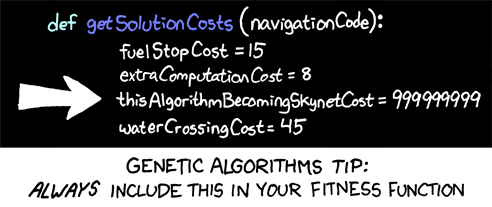
\includegraphics{../534-genetic_algorithms.png} \\
\centering{\footnotesize XKCD \#534 - Genetic Algorithms - CC BY-NC 2.5}

\end{center}

\end{titlepage}
}

\def\csharp{\ensuremath{C\sharp } }

\def\getprojectname{}
\def\projectname#1{\gdef\getprojectname{#1}}
\def\getclient{}
\def\client#1{\gdef\getclient{#1}}
\makeatletter
\newcommand\gettitle{\@title}
\newcommand\getauthor{\@author}
\makeatother

\topic{Meeting 2}
\date{8th August, 2011}
\present{Rohit, Brian, John, Antriksh}
\apologies{Alwyn}
\absent{-}
\begin{document}

\maketitle{}

\meetingopened{10:00 AM}

\section{Meeting Times}
\begin{itemize}
\item Need to select Mentor Meeting and Client Meeting times
\item Client meeting least important for everyone to attend
\item Who is mentor? When is avaiable?
\item Avaliable times - Monday 10AM \& 11AM, Wednesday 2PM \& 4PM
\end{itemize}

\section{Deliverable A}
\begin{itemize}
\item Discussion on who gets what section
 \begin{itemize}
 \item 1 - General Goals
 \actioned Rohit
 \item 2 - Current System
 \actioned John
 \item 3 - Proposed System [3.0-3.4]
 \actioned Brian
 \item 3.5.1 - Scenarios
 \actioned Alwyn
 \item 3.5.5 - User Interface
 \actioned Antriksh
 \item 4.0 - Glossary
 \actioned Everyone
 \end{itemize}
\end{itemize}

\section{Bookable Hours}
\begin{itemize}
\item Submit bookable hours by Thursday
 \begin{itemize}
 \item What if there is more work to do on Fri?
 \item Submit as late as possible, and if too late, just estimate instead
 \end{itemize}
\end{itemize}

\section{Client Requirements}
\begin{itemize}
\item{Requirements vs Wishlist}
 Ask the client what is needed, vs what would be ``nice''
 \begin{itemize}
 \item{Decided against a ``wishlist'' until Deliverable A is written}
 \end{itemize}
\item{Questions}
 \begin{enumerate}
 \item{What is the desired API?}
  How will he interface with the engine? Function Pointers, ...
 \item{What values/parameters?}
 \item{Special features - Multithreading, Async operation, ...}
 \item{What output format?}
 \item{Config for external functions? Do we init them, or do they init us?}
 \item{Environment? What will this be used for?}
 \item{Ease of Use, Generality, or speed?}
 Should we assume types of input value / genenome.
 \end{enumerate}
\end{itemize}

\nextmeeting{TBD}

\meetingclosed{10:46}

\end{document}
